\documentclass[10pt,letterpaper]{hmcpset}
\usepackage[margin=1in]{geometry}
\usepackage{graphicx}
\usepackage{amsmath,amssymb}
\usepackage[T1]{fontenc}

\newcommand{\aln}[1]{\begin{align*} #1 \end{align*}} %fast align

\assignment{Hillar, Windfeldt Section 4 Problems}
\name{Max Comstock}
\class{Professor Omar}
\duedate{Summer 2014}

\begin{document}

\begin{problem}[1]
Write a proof of Lemma 4.2 without looking at the proof given in the paper.
\end{problem}

\begin{solution}
First, note that $h_{U\backslash\{i\}}^{d+1}$ contains all polynomials of degree $d+1$ in $U$ that do not contain $x_i$. We may then subtract this polynomial from $h_U^{d+1}$, leaving only the polynomials of degree $d+1$ that contain $x_i$. By dividing out $x_i$, this can be written
\aln{
	x_i h_U^d = h_U^{d+1} - h_{U\backslash\{i\}}^{d+1}.
}
By replacing the index $i$ with $j$, we also obtain
\aln{
	x_j h_U^d = h_U^{d+1} - h_{U\backslash\{j\}}^{d+1}.
}
Thus
\aln{
	(x_i - x_j) h_U^d &= x_i h_U^d - x_j h_U^d\\
	(x_i - x_j) h_U^d &= h_U^{d+1} - h_{U\backslash\{i\}}^{d+1} - \left(h_U^{d+1} - h_{U\backslash\{j\}}^{d+1} \right)\\
	(x_i - x_j) h_U^d &= h_{U\backslash\{j\}}^{d+1} - h_{U\backslash\{i\}}^{d+1}.
}
\end{solution}


\begin{problem}[2]
Verify Lemma 4.3 on the graph below (label the vertices however you like):
\begin{center}
	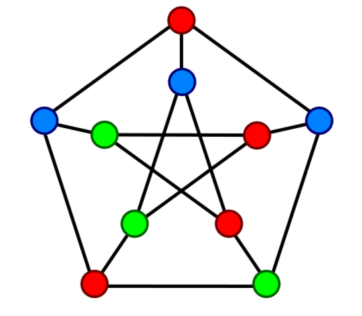
\includegraphics[width=2in]{3coloring.png}
\end{center}
\end{problem}

\begin{solution}
This has been verified.
\end{solution}


\begin{problem}[3]
Verify Lemma 4.4 on the graph in Problem 2. You will want to read Section 2 of the paper to know what a radical ideal is.
\end{problem}

\begin{solution}
This has been verified using Macaulay 2.
\end{solution}


\begin{problem}[4]
Read and understand the proof of Lemma 4.4.
\end{problem}



\end{document}
